\chapter{内存管理模块的 Rust 重构}

\section{重构需求与总体设计}

原系统的内存管理模块负责物理页分配、内核动态内存、用户空间、页表映射和交换区管理。在 C++ 版本中，这些功能主要由 PageManager、KernelPageManager、UserPageManager、MemoryDescriptor 和 SwapperManager 等对象承担，整体上延续了以内核页池、用户页池、分页和交换机制为基础的 Unix 教学系统设计。

系统启动后划定内核页池和用户页池边界，并初始化相应管理结构。进程创建和执行过程中需要申请用户页、建立页表映射，并在物理内存不足时借助交换区转移部分进程映像。内核运行期间还会频繁申请小块动态内存，用于进程控制块、缓冲区对象、文件对象和同步结构。原系统能够支撑这些基本需求，但分配逻辑主要围绕页级资源展开，对不同粒度的内存请求缺少分层处理。

原系统物理内存分配以页为基本单位，内核页池和用户页池分别维护可用内存区域。其基本方法是在预先划定的内存范围内记录空闲页块的起始地址和大小；分配时按页对齐请求，在空闲表中查找满足要求的连续区间；释放时将区间归还空闲表。该方法便于解释页式分配的基本思想，也容易与内核地址空间布局对应，但分配粒度较粗，对碎片控制和小对象分配支持有限。基于这一限制，重构版本引入 Buddy + Slab 分层分配结构，将页级资源管理和对象级分配分离。

Rust 重构遵循两个约束。其一，保留页式管理、内核与用户空间分离、交换区辅助运行等教学逻辑，避免重构后难以与原系统对应。其二，收紧资源管理边界，将页对象、地址类型和分配接口显式化。内存管理不可避免地涉及裸地址、页表和硬件资源，因此 unsafe 代码无法完全消除；重构重点在于限制 unsafe 边界，并在其上层使用类型系统、所有权和 RAII 风格封装表达资源关系。

这一章不把内存管理模块的所有函数逐一说明，而是集中讨论三处对系统影响较大的改动。第一处是物理页从“地址区间”变为“带状态的资源对象”，它决定 Buddy、Slab、页表和用户页之间能否共享一致的页状态。第二处是内核堆从单一页级分配扩展为 Buddy + Slab 分层分配，它直接影响内核对象的空间利用率和释放路径。第三处是页表、地址类型和交换区管理的重新组织，它们把原先散落在机器相关代码和进程管理流程中的地址关系收束到更明确的边界内。这些改动并不追求改变 Unix V6++ 的教学行为，而是使原有机制在 Rust 中具有更清楚的资源语义。

Rust 版本将内存管理拆分为若干子模块。page.rs 定义物理页对象 PhysPage、页集合 Pages 和页链表；page\_manager.rs 基于 Buddy 算法组织页分配器，并分别维护内核页和用户页两个实例；allocator.rs 接入全局分配器，在内核动态分配层面组合 Slab 与 Buddy；zone.rs 描述物理内存范围和页元数据数组；swapper\_manager.rs 负责交换区空间组织。各模块的职责如\cref{tab:mm-modules} 所示。

\begin{table}[htbp]
  \centering
  \caption{内存管理子模块功能说明表}\label{tab:mm-modules}
  \begin{tabular}{p{0.28\textwidth}p{0.62\textwidth}}
    \toprule
    \textbf{代表文件} & \textbf{主要功能} \\
    \midrule
    mm.rs & 组织并导出内存管理相关子模块，对外提供统一接口 \\
    page.rs & 定义 PhysPage、KernelPages、UserPages、页链表等基础数据结构，作为 Buddy 分配器和 Slab 分配器的共同基础 \\
    page\_manager.rs & 基于 Buddy 算法管理内核页池和用户页池，负责页块的初始化、分配与释放 \\
    allocator.rs & 接入全局分配器，按大小选择 Slab 或 Buddy 路径，完成内核动态内存分配 \\
    zone.rs & 描述物理内存范围，维护全部物理页的元数据数组，为页分配器提供页对象映射 \\
    swapper\_manager.rs & 管理交换区空闲区间，支持交换区空间的分配、释放与合并 \\
    kstack.rs & 为进程或内核执行流提供内核栈页封装，基于底层页分配器申请和回收栈空间 \\
    page\_table.rs & 定义页目录项、页表项及映射初始化逻辑，支持内核和用户空间的页表管理 \\
    \bottomrule
  \end{tabular}
\end{table}

\section{物理内存管理机制的重构}

在物理页数据结构设计上，Rust 版本首先重构物理页表示。每个物理页统一表示为 PhysPage 结构，其中包含链表链接、页块阶数、是否属于 Buddy 系统、是否用作 Slab 页等元信息。页对象内部还保留联合数据区，用于记录 Slab 页状态或用户页附加状态。由此，物理页不再只是可分配地址区间，也成为多个内存子系统共享的状态载体。

该设计将页状态集中到统一结构中，页分配器、Slab 分配器和地址空间管理模块可以围绕同一页对象协作。普通页、Slab 页和用户页不再依赖彼此分散的状态记录，而是通过页对象中的标志和附加数据区区分具体用途。对于教学系统而言，这种组织方式仍保留物理页作为基本资源单元的概念，同时使页与上层分配器之间的关系更清楚。

更重要的是，Rust 版本将连续页资源封装为 Pages、KernelPages 和 UserPages 等对象，使“申请到一组页”和“最终归还这组页”之间形成更明确的生命周期关系。原 C++ 版本中，调用者通常保存页起始地址或页框号，释放时再把这些数值交还给管理器；如果中途发生错误返回，释放责任需要依靠调用约定维持。重构后，页集合对象可以在 Drop 路径中承担回收责任，正常返回和错误返回都能落到同一套资源释放语义上。内核页和用户页仍然来自不同页池，但它们不再只是两个整数范围，而是由不同类型和不同管理器接口承载的资源。

这种封装并不意味着内存管理完全摆脱裸指针。页元数据数组、物理页内容清零、页表项写入和 DMA 共享缓冲区仍然需要触及底层地址。重构的实际作用是把这些操作限制在少数边界函数中，上层模块尽量传递页对象、页框号或地址范围，而不是在任意位置对整数地址做加减。对于内核代码而言，这种边界比单纯减少 unsafe 数量更重要，因为内存错误往往来自错误的所有权假设，而不只是来自某一处裸指针解引用。

地址与页框的类型安全抽象也是本次重构的重点。在原有 C++实现中，地址和页框大多直接以整数形式参与运算，这种方式虽然直观，但容易在不同语义层次间混用。Rust 版本引入了更明确的地址与页框抽象，例如PAddr 表示物理地址，PFN 表示物理页框号，PRange 表示物理地址范围。这些类型来自底层内存管理支持库，并在页分配器、页表和地址转换函数中被广泛使用。

类型化抽象使接口语义更明确。页框号、物理地址和地址范围不再以普通整数混用，调用者需要在类型层面区分不同地址语义。这样可以减少地址误传和单位误用，也使原本依赖经验维护的约束部分转化为编译期检查。

在页分配器实现上，Rust 版本引入了 Buddy 分配算法作为核心方案。新实现分别维护 KERNEL\_PAGE\_MANAGER 和 USER\_PAGE\_MANAGER 两个 Buddy 分配器，它们共享同一个物理内存区描述，但分别服务于内核页池和用户页池。初始化阶段，系统首先建立页的元数据区，然后根据原系统的地址划分，将内核页池和用户页池对应的物理范围注册到 Buddy 分配器中。

Buddy 分配算法将连续页块按照 2 的幂次组织。申请内存时，分配器根据请求大小计算阶数，并从对应或更高阶空闲链表中获得页块；释放时，根据伙伴关系尝试合并相邻空闲块。与原系统的线性空闲表相比，Buddy 的分裂和合并规则更稳定，适合为页表、内核栈和较大内核对象提供连续页资源。

Buddy 重构中需要处理的难点不在算法公式，而在页块状态的一致性。一个页块被拆分后，首个页对象需要记录阶数和 Buddy 归属，其余页不能再被当作独立空闲块重复释放；两个伙伴块合并时，又必须确认二者处于相同阶数、同属同一分配器且都处于空闲状态。若这些条件只靠调用者保证，错误通常会延迟到后续分配时表现为链表损坏或重复分配。Rust 版本把阶数、链表挂接和 Buddy 标志集中在页对象与分配器内部处理，使外部代码不直接拼装这些状态。

内核页池和用户页池分开管理后，还需要避免页资源跨池归还。对教学系统来说，内核页池与用户页池的边界不仅是地址范围划分，也对应不同的使用场景：内核页可能承载页表、内核栈和 Slab 页，用户页则参与进程映像和换入换出。Rust 版本在类型和管理器实例上同时保留这种区别，释放路径必须回到相应分配器。这一设计没有改变原系统“内核资源不从用户页池取、用户映像不占用内核页池”的基本策略，但使该策略在接口层更不容易被绕过。

\begin{figure}[htbp]
  \centering
  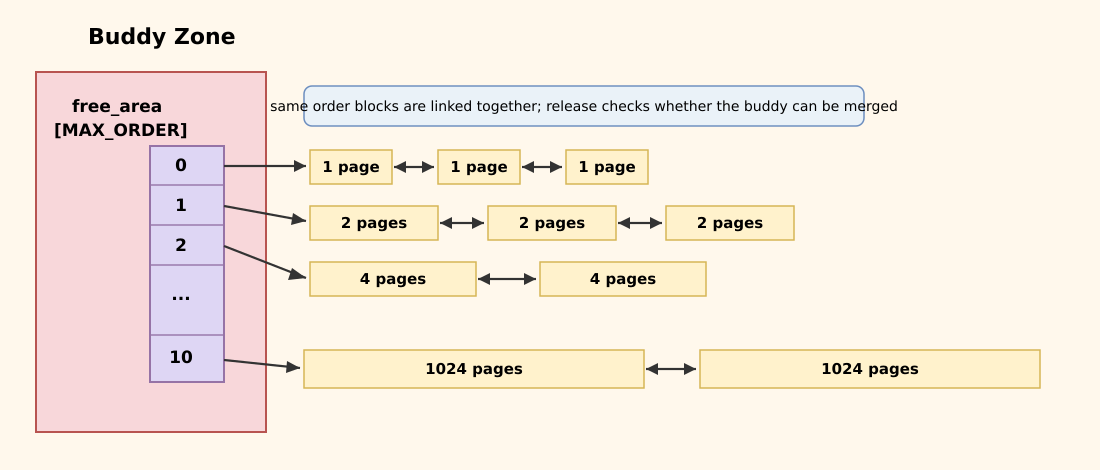
\includegraphics[width=0.72\textwidth]{figures/3/buddy_zone.svg}
  \caption{Buddy 分配算法的组织方式}
\end{figure}

\begin{figure}[htbp]
  \centering
  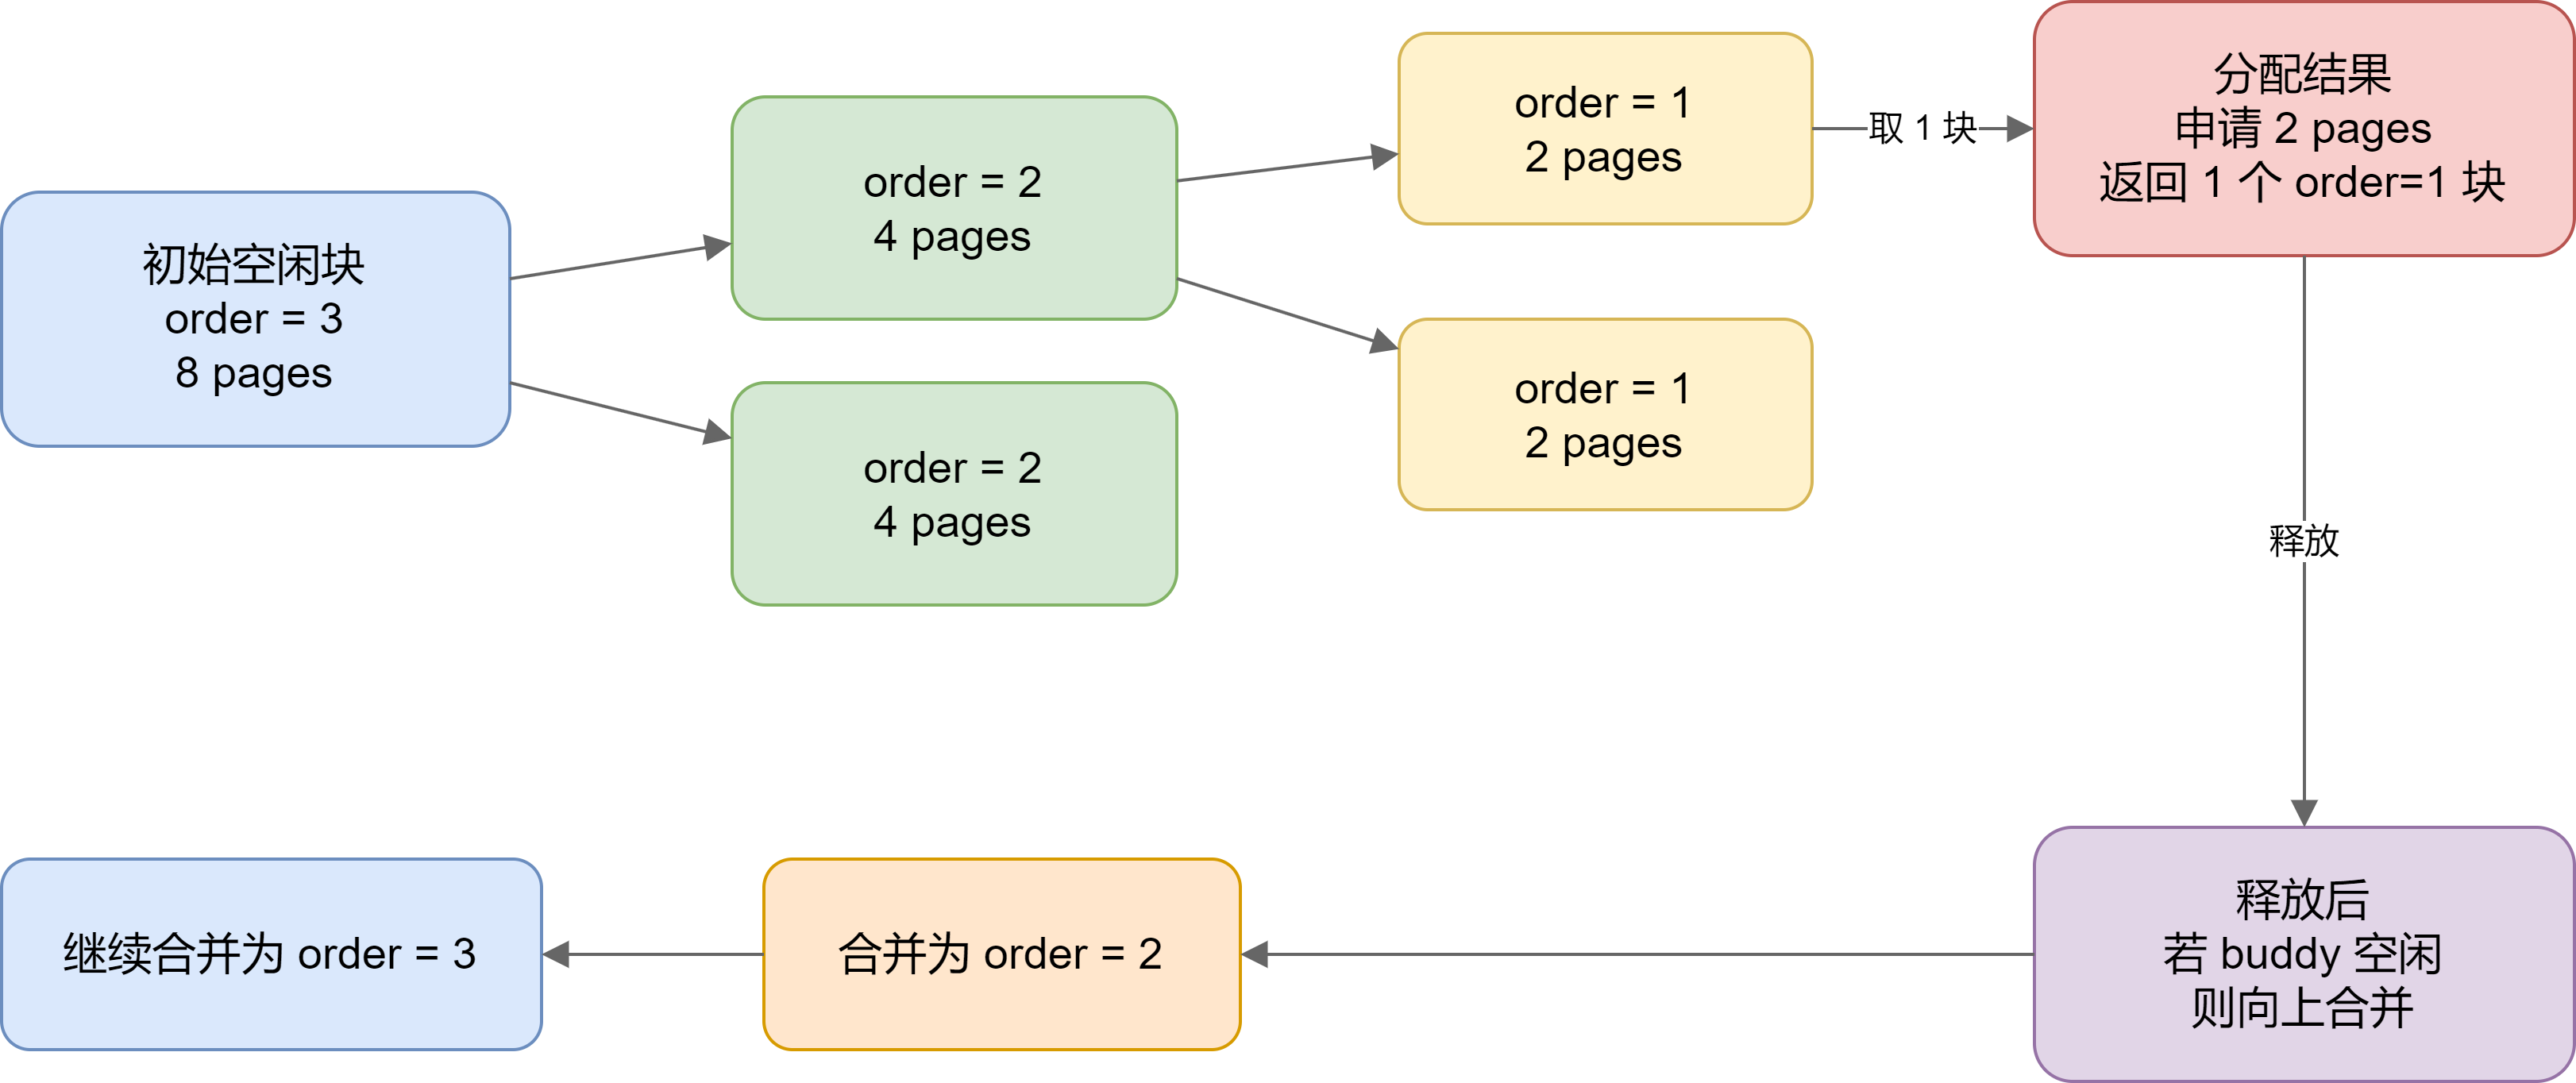
\includegraphics[width=0.68\textwidth]{figures/3/1buddy.png}
  \caption{Buddy 分配算法的分配流程}
\end{figure}

内核页池方面，Rust 版本延续了原系统内核页池和用户页池分离的设计，但在实现上更明确地将两者作为两个独立的分配器实例。内核页池主要服务于内核堆、页表、内核栈和其他内核内部对象；用户页池则主要用于进程地址空间和用户页分配。这样的划分符合原系统的运行模式。

这种划分延续了原系统中内核资源和用户资源分离管理的思想，也使内核堆、用户地址空间和进程换入换出等机制具有更明确的资源基础。与原实现相比，Rust 版本在接口层面更清楚地区分了两类页资源。

\section{内核堆与 Slab 分配机制重构}

操作系统内核中的动态内存请求并不总是以整页为单位出现。大量内核对象的大小都远小于一个页，例如链表节点、文件对象、页表辅助结构、同步原语或状态描述结构等。如果继续像原系统那样主要依赖页级分配来处理所有动态内存请求，就会造成较大的内部碎片，同时也会降低小对象分配和释放的效率。

因此，页分配器只能作为底层资源管理机制，内核堆还需要面向小对象的分配策略。Rust 版本在 Buddy 之上引入 Slab 分配器，底层按页管理物理资源，上层在页内切分固定大小槽位，从而降低小对象分配造成的内部碎片。

在当前实现中，Slab 分配器通过内核全局分配器接入系统。全局分配器实现 GlobalAlloc 接口，并根据分配请求大小决定采用哪种策略。当申请大小不超过 2048 字节时，请求交由SLAB\_ALLOCATOR 处理；当申请大小超过这一阈值时，则直接从 Buddy 分配器获取整页或多页块。这样做的目的是把小对象分配和页分配区分开来，使不同粒度的请求都能以更合适的方式处理。

Slab 分配器本身并不直接管理底层物理页，而是通过 SlabPageAlloc 接口向Buddy 系统申请新的页作为 Slab 页。当系统需要新的 Slab 页时，先从内核 Buddy 分配器中取出一个 0 阶页，再调用页对象上的初始化逻辑建立空闲槽位结构。随后，Slab分配器在该页内部管理固定大小的小对象槽位，并维护页内已分配对象数和空闲链表指针等状态。这样的实现方式体现了上层对象分配器依赖下层页分配器供页的分层结构。

为了支持 Slab 分配器运行，页对象中专门维护了与 Slab 相关的状态，例如空闲槽位链表指针和当前已分配对象计数。在 Rust 版本中，物理页不仅是被动的存储单元，而是主动参与到对象分配过程中的状态载体。当一个页被用作 Slab 页后，它会记录自身的槽位使用情况，供分配器后续快速复用。

对象级分配状态被绑定到页对象之后，页与页内槽位的关系更容易追踪。该实现也说明了内核堆通常不直接为每个小对象申请整页，而是在页级资源之上建立对象缓存，以改善空间利用率和分配成本。

Slab 分配路径还需要处理对齐和对象大小分类。内核对象虽然普遍小于一页，但不同对象对对齐有不同要求，若只按请求字节数简单切分页内空间，可能导致后续结构体访问不满足对齐约束。Rust 版本通过全局分配器接收 Layout 信息，根据大小和对齐要求选择合适的 Slab 类别；无法放入 Slab 的请求再退回 Buddy 页分配。这使内核中的 Box、Vec 等 Rust 容器可以接入同一套底层分配路径，而不需要每个模块分别维护临时内存池。

释放路径同样是 Slab 重构需要关注的部分。小对象释放时，分配器必须找到对象所在页，并把槽位重新挂回该 Slab 页的空闲链表；当页内对象全部释放后，该页才可能从 Slab 层回收到 Buddy 层。这里的边界如果处理不清，容易出现页仍被 Slab 持有却被 Buddy 再次分配的问题。重构后，Slab 页状态记录在 PhysPage 中，分配器根据页对象判断其用途和占用情况，减少了跨层释放时依赖外部约定的情况。

Buddy 与 Slab 在新系统中并不是相互独立的两套机制，而是上下层协同工作的整体。Buddy 负责管理物理页这一粗粒度资源，是整个内存分配体系的基础；Slab 则建立在 Buddy 提供的页之上，面向小对象实现细粒度分配。对于较大的内存请求，系统直接从 Buddy 获取页块；对于较小的内存请求，则从 Slab 页中分配对象槽位。释放时也按照相同层次返回对应资源。

\begin{figure}[htbp]
  \centering
  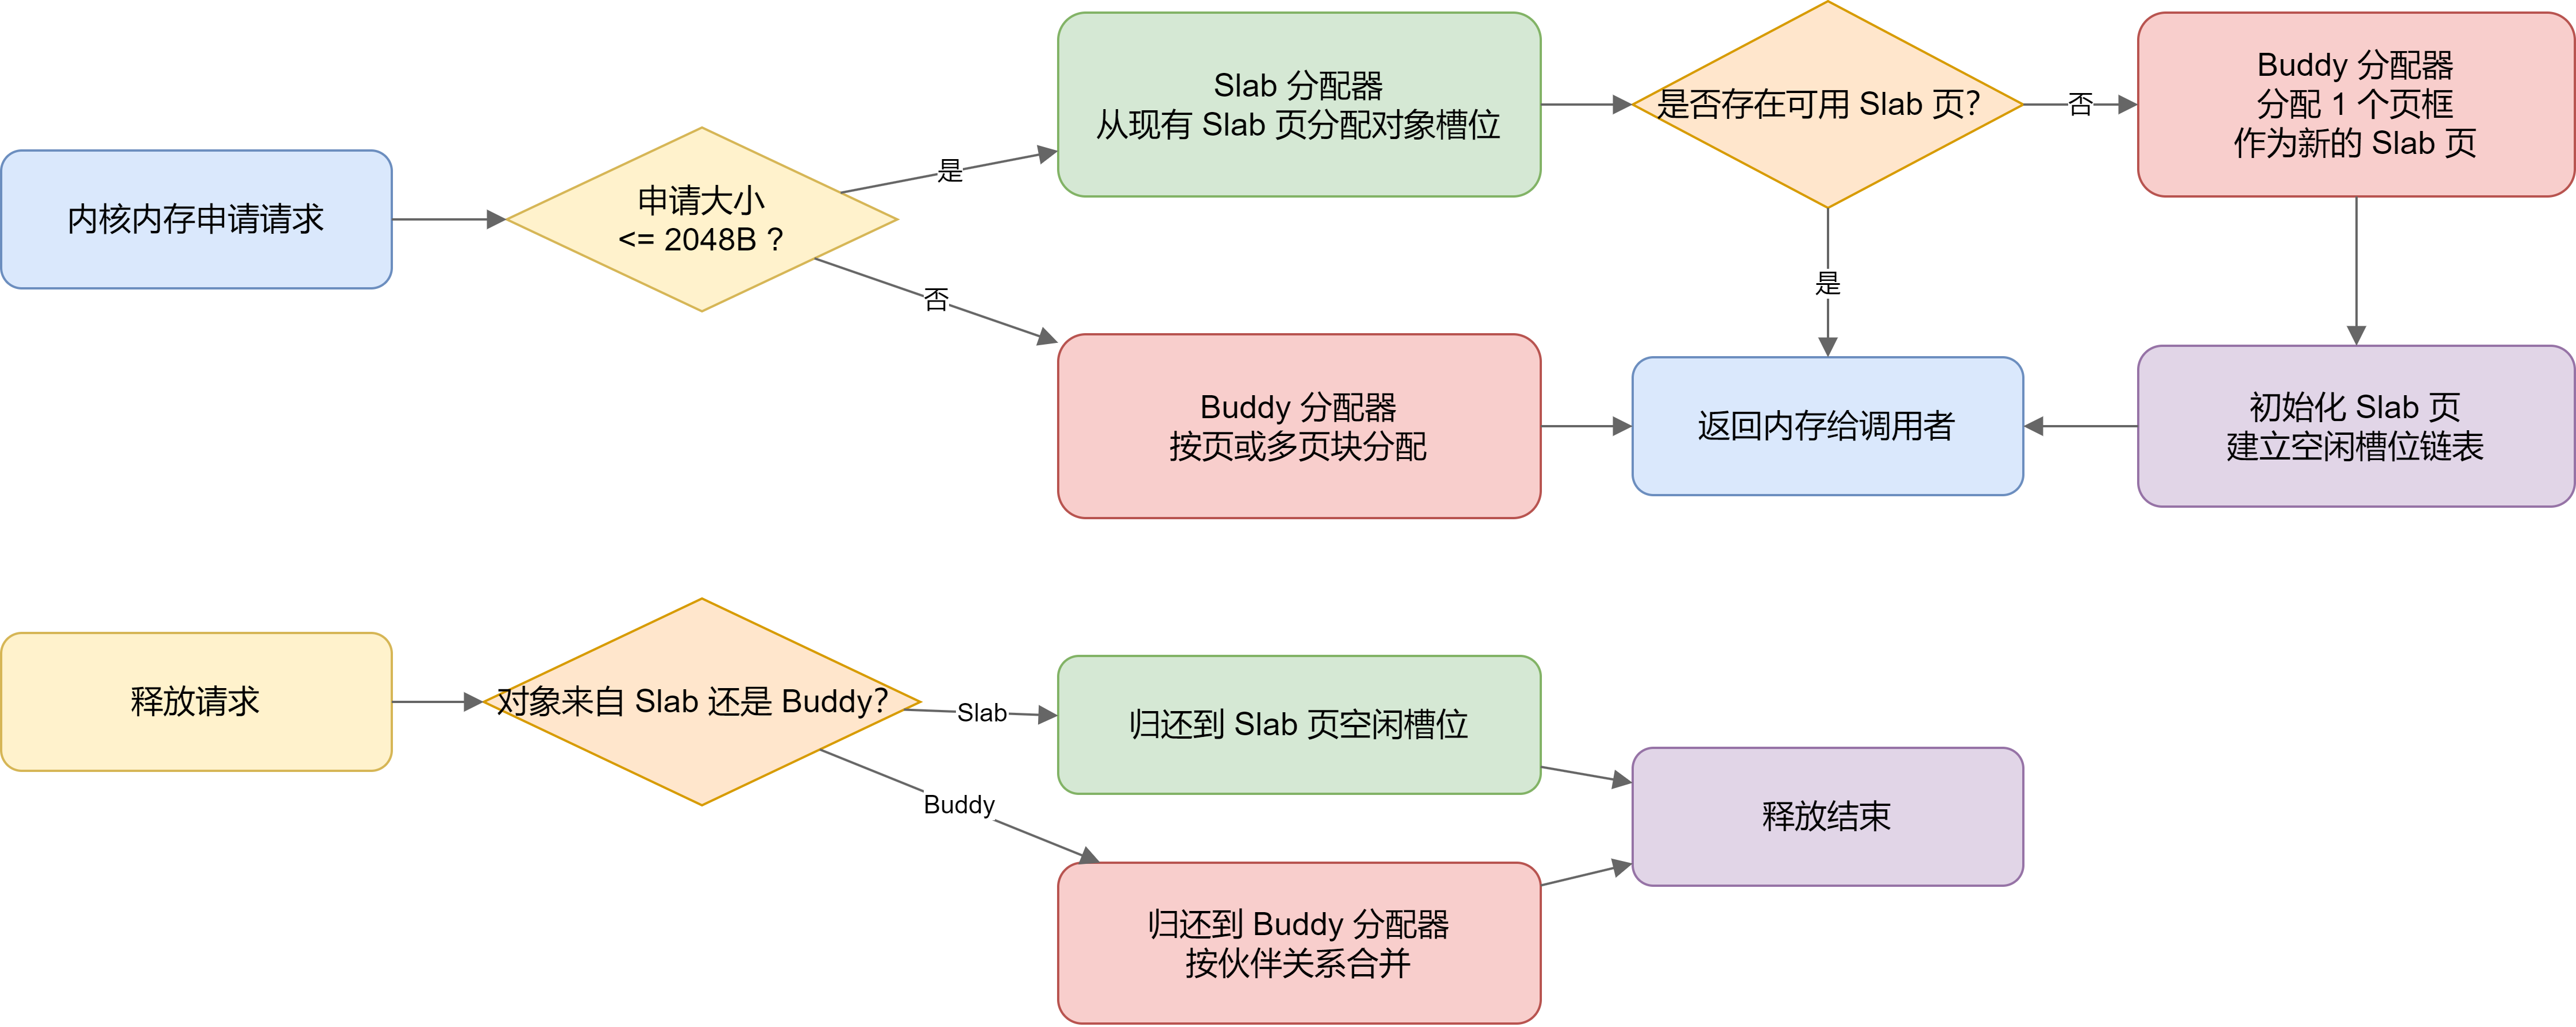
\includegraphics[width=0.72\textwidth]{figures/3/2buddyslab.png}
  \caption{Buddy 和 Slab 的协同分配}
\end{figure}

该协同机制覆盖了大块连续页和小对象两类场景。Buddy 负责页框资源，Slab 负责页内对象，二者之间通过明确接口传递页资源。相较于单一页级分配策略，这种分层结构更适合内核动态分配，也使分配路径更便于分析。

\section{页表与地址空间管理的重构}

Rust 版本定义 PageDirectoryEntry、PageTableEntry、PageDirectory 和 PageTable 等结构，并使用 bitflags 封装页项属性位，例如存在位、可写位、用户位和大页位。与原系统中的位域结构和直接位操作相比，该表示方式更便于在接口层表达页表项语义。

这部分重构主要将原有 IA32 分页机制迁移到 Rust 表示，而不是重新设计地址空间模型。其作用在于减少 C++ 机器相关代码的残留，并使页表逻辑能够与新的地址类型和页对象抽象衔接。

Rust 版本保留了原系统的基本地址空间布局：内核映射位于高地址空间，用户空间位于低地址区域，并通过固定数量的用户页表建立进程可见的虚拟地址空间。在初始化过程中，系统会设置内核页目录项、建立内核页表映射，并初始化用户页表数组。这部分实现更多是在 Rust 中复现原有 IA32 系统的地址空间组织策略，而非重新设计全新的虚拟内存模型。

在进程切换过程中，内核需要能够访问当前进程对应的用户结构和相关映射信息。Rust 版本中，系统通过修改内核页表中特定页表项，使其指向当前进程对应的页框，并在修改后刷新页目录，从而实现对当前进程用户结构映射的切换。这一机制延续了原系统的基本思路，但通过 Rust 提供了更统一的接口实现。

页表重构的实际难点在于同时面对两套约束。一方面，页表项必须精确符合 IA32 硬件格式，存在位、写权限、用户权限和页框地址不能被抽象层破坏；另一方面，内核上层又希望以代码段、数据段和栈段等逻辑概念描述用户空间。Rust 版本在这两者之间保留明确分界：底层页表结构负责位级编码和刷新操作，MemoryDescriptor 等上层结构负责描述进程地址空间布局。这样，上层扩展用户空间或调整段边界时，不需要直接操作页目录项中的每一位。

这种分界也为后续 RISC-V 迁移提供了参照。IA32 与 RISC-V 的页表层级、权限位和控制寄存器均不同，但用户空间需要表达的代码段、数据段、栈段和当前进程上下文访问关系基本一致。第 5 章中的 Sv39 适配正是在这一思路下完成：硬件页表结构可以替换，上层地址空间管理逻辑尽量保持稳定。换言之，第 3 章的页表重构并不是孤立的 Rust 改写，而是在为跨架构迁移保留可替换的机器相关边界。

\section{交换管理机制的重构}

原系统通过预留交换区来支持进程映像的换出与换入，以在物理内存不足时维持系统运行。Rust 版本保留了这一总体思想，但在交换区的内部管理方式上进行了重构。当前实现中，交换区由一个空闲区间表来描述，每个区间记录起始位置和大小，系统初始化时将整片交换区作为一个大的空闲区域加入管理结构。

这种做法将交换区明确建模为连续空间资源，而不是把分配状态分散嵌入换入换出流程。空闲区间、分割和合并逻辑集中后，交换区管理更容易审查，也便于后续替换分配策略。

在交换区分配时，系统会遍历当前空闲区间表，寻找第一个能够满足请求大小的区间。如果找到的区间大于请求大小，则从区间起始处分割出所需部分，并缩减剩余空闲区间；如果大小刚好匹配，则直接将该区间从空闲表中移除。释放时则按照地址顺序将区间插回，并尝试与前后相邻空闲区间合并，以减少碎片。这一实现在算法上并不复杂，优点在于逻辑明确、可验证性较好，并且与 Rust 的数据结构表达方式比较契合。相比原系统中更偏传统过程式的写法，新的交换区分配器在结构上更容易维护，也更便于后续替换为更复杂的管理策略。

Rust 版本没有改变交换机制的用途，仍然为内存不足时的进程换出和换入提供磁盘空间。变化主要体现在实现组织上：交换区被视为独立资源，空闲区间状态由专门结构维护，分配、释放和合并逻辑显式呈现。与 Buddy + Slab 相比，交换区重构更多体现为对原有机制的结构化表达。

交换区管理虽然不如页分配和 Slab 分配频繁，但它与进程生命周期关系紧密。进程换出时，系统需要为连续进程映像找到足够交换空间；换入或进程退出后，又必须把对应区间归还。若交换区碎片不能及时合并，系统可能在总空闲空间仍然足够时无法找到连续区间。重构后的区间表保持按地址顺序插入，释放时立即检查前后相邻区间，目的就是让这种碎片问题尽量在释放路径中被处理，而不是累积到下一次分配失败时才暴露。

\section{本章小结}

本章分析了 Unix V6++ 内存管理模块的 Rust 重构。重构没有改变以页为核心、结合分页和交换机制支撑进程运行的基本思想，而是在此基础上重新组织页对象、页分配器、内核堆和交换区管理逻辑。Buddy + Slab 构成新的分层分配框架，改善了原系统页级分配较为粗粒度的问题；类型化地址、页对象状态和显式交换区管理则使模块边界和资源关系更加清楚。上述变化为后续文件系统对象管理和 RISC-V 地址空间适配提供了基础。
